%Este trabalho está licenciado sob a Licença Atribuição-CompartilhaIgual 4.0 Internacional Creative Commons. Para visualizar uma cópia desta licença, visite http://creativecommons.org/licenses/by-sa/4.0/deed.pt_BR ou mande uma carta para Creative Commons, PO Box 1866, Mountain View, CA 94042, USA.

\chapter{Multiprocessamento (MP)}\label{cap_mp}
\thispagestyle{fancy}

Neste capítulo, vamos estudar aplicações da computação paralela em arquitetura de memória compartilhada. Para tanto, vamos discutir código C/C++ com a API \href{https://www.openmp.org/}{OpenMP}.

\section{Olá, Mundo!}\label{sec_ola_cap_mp}

A computação paralela com MP inicia-se por uma instância de processamento \emph{thread master}. Todas as instâncias de processamento disponíveis (\emph{threads}) leem e escrevem variáveis compartilhadas. A ramificação ({\it fork}) do processo entre os {\it threads} disponíveis é feita por instrução explícita no início de uma região paralela do código. Ao final da região paralela, todos os {\it threads} sincronizam-se ({\it join}) e o processo segue apenas com o {\it thread master}. Veja a Figura \ref{fig:mpwf}.

\begin{figure}[H]
  \centering
  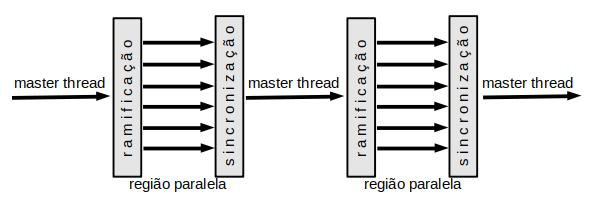
\includegraphics[width=0.7\textwidth]{./cap_mp/dados/fig_mpwf/mpwf}
  \caption{Fluxograma de um processo MP.}
  \label{fig:mpwf}
\end{figure}

Vamos escrever nosso primeiro programa MP. O Código \verb+ola.cc+ inicia uma região paralela e cada instância de processamento escreve ``Olá'' e identifica-se.

\lstinputlisting[title={Código: ola.cc}]{cap_mp/dados/cc_ola/ola.cc}

Na linha 4, o API OpenMP é incluído no código. A região paralela vale dentro do escopo iniciado pela instrução
\begin{verbatim}
# pragma omp parallel
\end{verbatim}
i.e., entre as linhas 12 e 17. Em paralelo, cada {\it thread} registra seu número de identificação na variável \verb+id+, veja a linha 14. Na linha 16, escrevem a saudação, identificando-se.

Para compilar este código, digite no terminal
\begin{verbatim}
$ g++ -fopenmp ola.cc
\end{verbatim}

Ao compilar, um executável \verb+a.out+ será criado. Para executá-lo, basta digitar no terminal:
\begin{verbatim}
$ a.out
\end{verbatim}

Ao executar, devemos ver a saída do terminal como algo parecido com\footnote{O código foi rodado em uma máquina Quadcore com 4 {\it threads}.}
\begin{verbatim}
Processo 0, olá!
Processo 3, olá!
Processo 1, olá!
Processo 2, olá!
\end{verbatim}

A saída irá depender do número de {\it threads} disponíveis na máquina e a ordem dos {\it threads} pode variar a cada execução. Execute o código várias vezes e analise as saídas!

\begin{obs}
  As variáveis declaradas dentro de uma região paralela são privadas de cada {\it threads}. As variáveis declaradas fora de uma região paralela são globais, sendo acessíveis por todos os {\it threads}.
\end{obs}

\subsection*{Exercícios resolvidos}

\begin{exeresol}
  O número de instâncias de processamento pode ser alterado pela variável do sistema \verb+OMP_NUM_THREADS+. Altere o número de {\it threads} para 2 e execute o Código ola.cc.
\end{exeresol}
\begin{resol}
  Para alterar o número de {\it threads}, pode-se digitar no terminal
\begin{verbatim}
$ export OMP_NUM_THREADS=2
\end{verbatim}
  Caso já tenha compilado o código, não é necessário recompilá-lo. Basta executá-lo com
\begin{verbatim}
$ ./a.out
\end{verbatim}
  A saída deve ser algo do tipo
\begin{verbatim}
Olá, processo 0
Olá, processo 1
\end{verbatim}
\end{resol}

\begin{exeresol}
  Escreva um código MP para ser executado com 2 {\it threads}. O {\it master thread} deve ler dois números em ponto flutuante. Então, em paralelo, um dos {\it threads} deve calcular a soma dos dois números e o outro thread deve calcular o produto.
\end{exeresol}
\begin{resol}
\lstinputlisting[title={Código: sp.cc}]{cap_mp/dados/cc_exeresol_sp/sp.cc}  
\end{resol}

\subsection*{Exercícios}

\begin{exer}
  Defina um número de {\it threads} maior do que o disponível em sua máquina. Então, rode o código \verb+ola.cc+ e analise a saída. O que você observa?
\end{exer}

\begin{exer}
  Modifique o código \verb+ola.cc+ de forma que cada {\it thread} escreva na tela ``Processo ID de NP, olá!'', onde ID é a identificação do {\it thread} e NP é o número total de {\it threads} disponíveis. O número total de {\it threads} pode ser obtido com a função OpenMP
\begin{verbatim}
omp_get_num_threads();
\end{verbatim}
\end{exer}

\begin{exer}
  Faça um código MP para ser executado com 2 threads. O {\it master thread} deve ler dois números $a$ e $b$ não nulos em ponto flutuante. Em paralelo, um dos {\it thread} de computar $a-b$ e o outro deve computar $a/b$. Por fim, o {\it master thread} deve escrever $(a-b) + (a/b)$.
\end{exer}

\begin{exer}\label{exer:cc_exer_Ax}
  Escreva um código MP para computar a multiplicação de uma matriz $n\times n$ com um vetor de $n$ elementos. Inicialize todos os elementos com números randômicos em ponto flutuante. Ainda, o código deve ser escrito para um número arbitrário $m>1$ de instâncias de processamento. Por fim, compare o desempenho do código MP com uma versão serial do código.
\end{exer}

\begin{exer}\label{exer:cc_exer_AB}
  Escreva um código MP para computar o produto de uma matriz $n\times m$ com uma matriz de $m\times n$ elementos, com $n \geq m$. Inicialize todos os elementos com números randômicos em ponto flutuante. Ainda, o código deve ser escrito para um número arbitrário $m>1$ de instâncias de processamento. Por fim, compare o desempenho do código MP com uma versão serial do código.
\end{exer}

\section{Construtores básicos}\label{cap_mp_sec_cb}

\subsection{Variáveis privadas e variáveis compartilhadas}

Vamos analisar o seguinte código.

\lstinputlisting[title={Código: vpc.cc}]{cap_mp/dados/cc_vpc/vpc.cc}

Qual seria a saída esperada? Ao rodarmos este código, veremos uma saída da forma
\begin{verbatim}
Processo 0/4
Processo 2/4
Processo 3/4
Processo 3/4
\end{verbatim}
Isto ocorre por uma situação de \emph{condição de corrida} (\emph{race condition}) entre os {\it threads}. As variáveis \verb+tid+ e \verb+nt+ foram declaradas antes da região paralela e, desta forma, são \emph{variáveis compartilhadas} (\emph{shared variables}) entre todos os {\it threads} na região paralela. Os locais na memória em que estas as variáveis estão alocadas é o mesmo para todos os {\it threads}.

A condição de corrida ocorre na linha 11. No caso da saída acima, as instâncias de processamento 1 e 3 entraram em uma condição de corrida no registro da variável \verb+tid+.

\begin{obs}
  Devemos estar sempre atentos a uma possível condição de corrida. Este é um erro comum no desenvolvimento de códigos em paralelo.
\end{obs}

Para evitarmos a condição de corrida, precisamos tornar a variável \verb+tid+ privada na região paralela. I.e., cada {\it thread} precisa ter uma variável \verb+tid+ privada. Podemos fazer isso alterando a linha 9 do código para
\begin{verbatim}
#pragma omp parallel private(tid)
\end{verbatim}
Com essa alteração, a saída terá o formato esperado, como por exemplo
\begin{verbatim}
Processo 0/4
Processo 3/4
Processo 2/4
Processo 1/4
\end{verbatim}
Faça a alteração e verifique!

\begin{obs}
  A diretiva \verb+#pragma omp parallel+ também aceita as instruções:
  \begin{itemize}
  \item \verb+default(private|shared|none)+: o padrão é \verb+shared+;
  \item \verb+shared(var1, var2, ..., varn)+: para especificar explicitamente as variáveis que devem ser compartilhadas. 
  \end{itemize}
\end{obs}

\subsection{Laço e Redução}

Vamos considerar o problema de computar
\begin{equation}
  s = \sum_{i=0}^{99999999} 1
\end{equation}
em paralelo com $np$ {\it threads}. Começamos analisando o seguinte código

\lstinputlisting[title={Código: soma0.cc}]{cap_mp/dados/cc_soma/soma0.cc}

Ao executarmos este código com $nt > 1$, vamos ter saídas erradas. Verifique! Qual o valor esperado?

O erro do código está na \emph{condição de corrida} ({\it race condition}) na linha 20. Esta é uma operação, ao ser iniciada por um {\it thread}, precisa ser terminada pelo {\it thread} antes que outro possa iniciá-la. Podemos fazer adicionando o construtor
\begin{verbatim}
#pragma omp critical
\end{verbatim}
imediatamente antes da linha de código \verb-s += i;-. O código fica como segue, verifique!

\lstinputlisting[title={Código: soma1.cc}]{cap_mp/dados/cc_soma/soma1.cc}

Esta abordagem evita a condição de corrida e fornece a resposta esperada. No entanto, ela acaba serializando o código, o qual é será muito mais lento que o código serial. Verifique!

\begin{obs}
  A utilização do construtor
\begin{verbatim}
#pragma omp critical
\end{verbatim}
  reduz a performance do código e só deve ser usada quando realmente necessária.
\end{obs}

Uma alternativa é alocar as somas parciais de cada {\it thread} em uma variável privada e, ao final, somar as partes computadas. Isto pode ser feito com o seguinte código. Verifique!

\lstinputlisting[title={Código: soma2.cc}]{cap_mp/dados/cc_soma/soma2.cc}

Este último código pode ser simplificado usando o construtor
\begin{verbatim}
#pragma omp for
\end{verbatim}
Com este construtor, o laço do somatório pode ser automaticamente distribuindo entre os {\it threads}. Verifique o seguinte código!

\lstinputlisting[title={Código: somafor.cc}]{cap_mp/dados/cc_soma/somafor.cc}

Mais simples e otimizado, é automatizar a operação de redução (no caso, a soma das somas parciais) adicionado
\begin{verbatim}
reduction(+: s)
\end{verbatim}
ao construtor que inicializa a região paralela. Verifique o seguinte código!

\lstinputlisting[title={Código: soma.cc}]{cap_mp/dados/cc_soma/soma.cc}

\begin{obs}
  A instrução de redução pode ser usada com qualquer operação binária aritmética (\verb=+=, \verb=-=, \verb=/=, \verb=*=), lógica (\verb=&=, \verb=|=) ou procedimentos intrínsecos (\verb=max=, \verb=min=).
\end{obs}

\subsection{Sincronização}

A sincronização dos {\it threads} deve ser evitada sempre que possível, devido a perda de performance em códigos paralelos. Atenção, ela ocorre implicitamente no término da região paralela!

\subsubsection{Barreira}

No seguinte código, o {\it thread} 1 é atrasado em 1 segundo, de forma que ele é o último a imprimir. Verifique!

\lstinputlisting[title={Código: sinc0.cc}]{cap_mp/dados/cc_sinc/sinc0.cc}

Agora, podemos forçar a sincronização dos {\it threads} usando o construtor
\begin{verbatim}
#pragma omp barrier
\end{verbatim}
em uma determinada linha do código. Por exemplo, podemos fazer todos os {\it threads} esperarem pelo {\it thread} 1 no código acima. Veja a seguir o código modificado. Teste!

\lstinputlisting[title={Código: sinc1.cc}]{cap_mp/dados/cc_sinc/sinc1.cc}

\subsubsection{Seção}

O construtor \verb+sections+ pode ser usado para determinar seções do código que deve ser executada de forma serial apenas uma vez por um único {\it thread}. Verifique o seguinte código.

\lstinputlisting[title={Código: secao.cc}]{cap_mp/dados/cc_secao/secao0.cc}

No código acima, o primeiro {\it thread} que alcançar a linha 19 é o único a executar a seção 1 e, o primeiro que alcançar a linha 25 é o único a executar a seção 2.

Observe que ocorre a sincronização implícita de todos os {\it threads} ao final do escopo \verb+sections+. Isso pode ser evitado usando a cláusula \verb+nowait+, i.e. alterando a linha 16 para
\begin{verbatim}
# pragma omp sections nowait
\end{verbatim}
Teste!

\begin{obs}
  A clausula \verb+nowait+ também pode ser usado com o construtor \verb+for+, i.e.
\begin{verbatim}
#pragma omp for nowait
\end{verbatim}
\end{obs}

Para uma região contendo apenas uma seção, pode-se usar o construtor
\begin{verbatim}
#pragma omp single
\end{verbatim}
Isto é equivalente a escrever
\begin{verbatim}
#pragma omp sections
  #pragma omp section
\end{verbatim}

\subsection*{Exercícios Resolvidos}

\begin{exeresol}\label{exeresol:produto_escalar}
  Escreva um código MP para computar o produto escalar entre dois vetores de $n$ pontos flutuantes randômicos.
\end{exeresol}
\begin{resol}
  Aqui, vamos usar o suporte a vetores e números randômicos do pacote de computação cientifica \href{https://www.gnu.org/software/gsl/}{GSL}. A solução é dada no código a seguir.

  \lstinputlisting[title={Código: secao.cc}]{cap_mp/dados/cc_prodesc/prodesc.cc}

  Para compilar o código acima, digite
\begin{verbatim}
$ g++ -fopenmp prodesc.cc -lgsl -lgslcblas
\end{verbatim}
\end{resol}

\emconstrucao

\subsection*{Exercícios}

\begin{exer}
  Considere o seguinte código
  \begin{lstlisting}
    int tid = 10;
    #pragma omp parallel private(tid)
    {
      tid = omp_get_thread_num();
    }
    printf("%d\n", tid);
  \end{lstlisting}
  Qual o valor impresso?
\end{exer}

\begin{exer}\label{exer:cc_trap}
  Escreva um código MP para computar uma aproximação para
  \begin{equation}
    I = \int_{-1}^{1} e^{-x^2}\,dx
  \end{equation}
  usando a \href{https://phkonzen.github.io/notas/MatematicaNumerica/cap_integr_sec_int_comp.html}{regra composta do trapézio} com $n$ subintervalos uniformes.
\end{exer}

\begin{exer}\label{exer:cc_simp}
  Escreva um código MP para computar uma aproximação para
  \begin{equation}
    I = \int_{-1}^{1} e^{-x^2}\,dx
  \end{equation}
  usando a \href{https://phkonzen.github.io/notas/MatematicaNumerica/cap_integr_sec_int_comp.html}{regra composta de Simpson} com $n$ subintervalos uniformes. Dica: evite sincronizações desnecessárias!
\end{exer}

\emconstrucao